\setauthor{Abdulrahman Al Sabagh}
\section{Strapi}
Strapi ist ein Headless \textbf{C}ontent \textbf{M}anagment \textbf{S}ystem (CMS),
welches eine vorgefertigte Benutzeroberfläche für Content-Creator
und auch für die Entwickler bereitstellt.

Durch den Einsatz von Strapi sind Inhalte und dafür notwendige technische Funktionalitäten
sehr einfach erstellbar.
\cite{strapi-vs-wordpress}


\subsection*{Welche eingebauten Funktionalitäten bietet Strapi für Entwickler und Content-Manager?}


Für die Entwickler werden folgende Funktionalitäten zur Verfügung gestellt:

\begin{itemize}
  \item fertige REST-Schnittstellen
  \item GraphQL Schnittstellen
  \item eine Benutzeroberfläche, wo die Struktur der Datenbank editiert werden kann
  \item eine eingebaute JWT Authentifizierung
  \item File Upload
  \item Query Engine API
  \item Entity Service API
  \item Plugin für Internationalisierung
  \item Plugin Store, mit dem sehr viele hilfreiche Plugins wie zum Beispiel OpenAPI installieren werden können
  \item Autorisierung und Rollenmanagement
\end{itemize}

\subsection{REST-Schnittstellen}
\label{subsec:rest}
Für jedes Modell werden die benötigten GET, POST, PUT und DELETE REST-Schnittstellen standardmäßig erstellt.
Jeder Endpoint unterstützt auch eine Menge von unterschiedlichen Parametern, welche den Aufbau des Responsebodys steuern können wie zum Beispiel.: filters, populate  und fields.
\cite{rest-query-parameters}
\subsection{Definition von Datenstruktur und Datenmodell}

Mit der Verwendung dieser Oberfläche kann man folgende Elemente erstellen:
\begin{itemize}
  \item Collection Types
  \item Single Types
  \item Components
\end{itemize}

\subsubsection{Collection Types}

''Collection types are content-types that can manage several entries.''
\cite{collection-types}

Mit der Verwendung von dieser Collection Types kann man die Struktur einer Tabelle bzw. einer Collection definieren.
Allerdings entspricht die Struktur der definierten SQL-Tabelle oder NoSQL-Collection nicht eins zu eins dem Collection Type.
Die speziellen Datentypen wie Files oder Custom Components werden nicht in der Datenbank als eine Tabellenspalte gespeichert.
Stattdessen werden die speziellen Typen in einer anderen Tabelle gespeichert.

Folgende Datentypen  werden von Strapi zur Verfügung gestellt:

\begin{figure}[H]
  \centering
  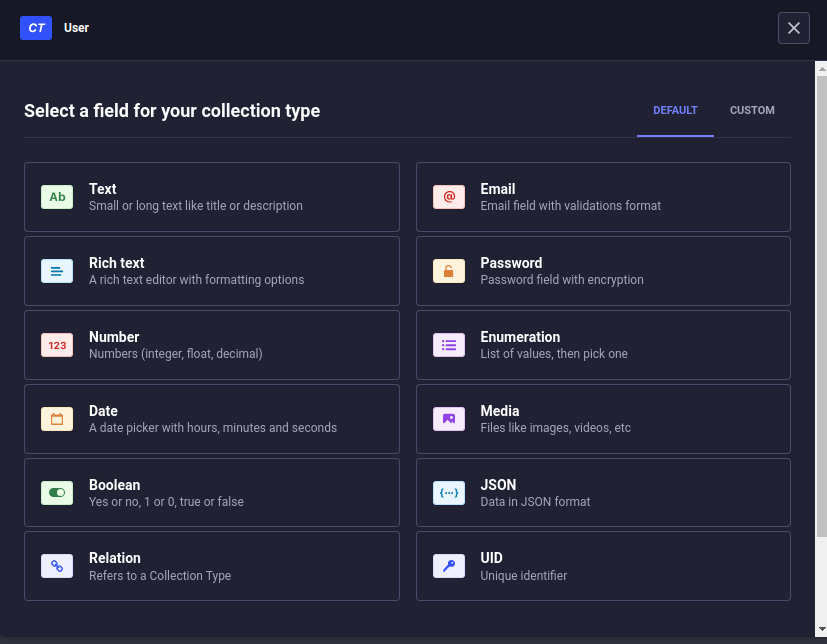
\includegraphics[width=\textwidth]{./pics/datatypes}
  \caption{Datentypen}
  \label{datatypes}
\end{figure}

Die Relationen zu anderen ''Collection Types'' werden von Strapi als ein Datentyp interpretiert.
Dieser unterstützt die Standardbeziehungen einer relationalen Datenbank zusätzlich zu bidirektionalen Beziehungen.
Bei den ''Many to Many'' Beziehungen ist die Erstellung eines zusätzlichen Collection Types, welcher als eine Assoziationstabelle dient, gar nicht nötig.
Die Assoziationstabellen werden von Strapi im Hintergrund generiert.

\begin{figure}[H]
  \centering
  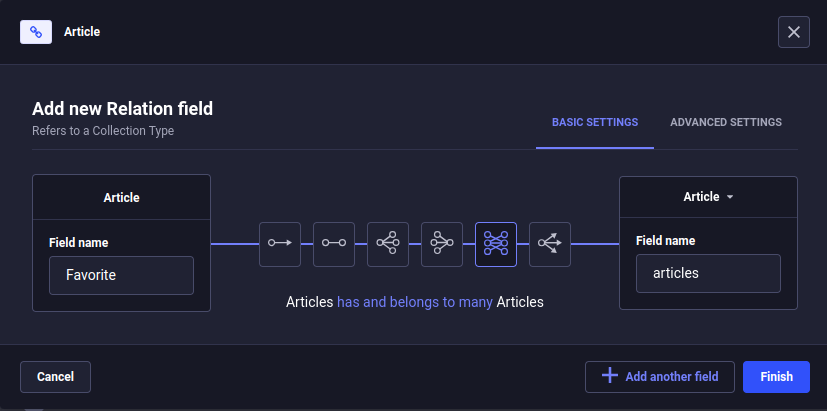
\includegraphics[width=\textwidth]{./pics/relations}
  \caption{Relationen}
  \label{relations}
\end{figure}

Zusätzlich zur Erstellung von Spalten haben Collection Types auch eine eingebaute Validierung, die man aktivieren kann.

\begin{figure}[H]

  \centering
  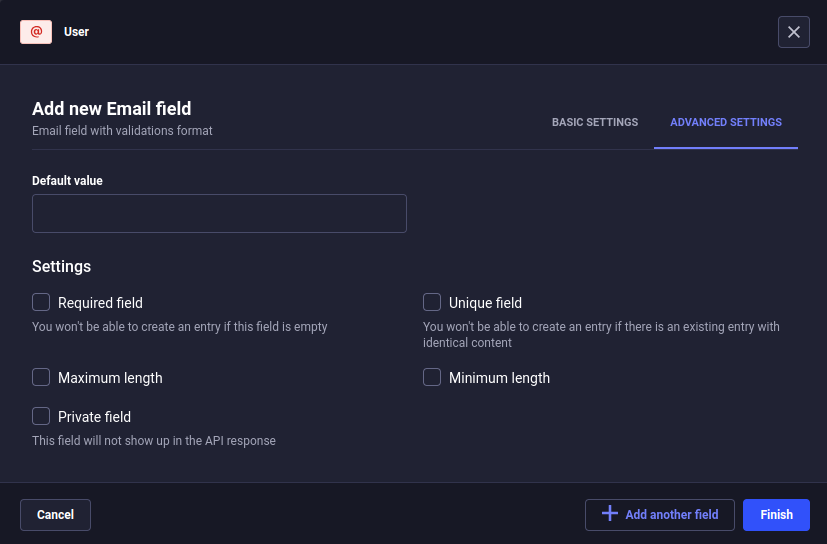
\includegraphics[width=\textwidth]{./pics/validation.png}
  \caption{validation}
  \label{validation}

\end{figure}

\subsubsection{Single Types}
\label{single-types}
''Single types are content-types that can only manage one entry''
\cite{collection-types}

\subsubsection*{Components}
''Components are a data structure that can be used in multiple collection types and single types.''
\cite{collection-types}


Es ist anzumerken, dass die Änderung der Struktur der Datenbank nur im ''Dev Mode'' funktionieren kann. In der produktiven Umgebung ist die Änderung der Tabellenstruktur nicht möglich.


\subsection{Query Engine API}
''The Strapi backend provides a Query Engine API to interact with the database layer at a lower level.
The Query Engine API should mostly be used by plugin developers and developers adding custom business logic
to their applications.''
\cite{query-engine-api}

Diese agiert als \textbf{O}bject \textbf{R}elational \textbf{M}apper (ORM) bzw. Query Builder, 
in der man SQL oder NoSQL Queries aus einem JS Code generieren kann. Die selektierte Spalten werden dann in JS-Objekten 
serialisiert.

\subsection{Entity Service API}
''The Strapi backend provides an Entity Service API, built on top of the Query Engine API.
The Entity Service is the layer that handles Strapi's complex data
structures like components and dynamic zones, and uses the Query Engine API
under the hood to execute database queries.''

Der Unterschied zwischen diesem Service und der Query Engine API liegt darin,
dass die Entity Service API nicht nur die SQL oder NoSQL Struktur einer
Tabelle bzw. einer Collection, sondern auch die besonderen Datentypen eines Strapi-Models wie zum Beispiel Files und Custom Components abfragen kann.
\cite{service-engine-api}
\subsection{File Upload}

Dabei ist das Wichtige, dass man Strapi so konfigurieren kann, dass es die Uploads für mehrere Bildschirme anpassen kann.
\begin{lstlisting}[caption=file upload config in strapi]
    export default ({ env }) => ({
        upload: {
          config: {
            breakpoints: {
              xlarge: 1920,
              large: 1000,
              medium: 750,
              small: 500,
              xsmall: 64
            },
          },
        },
      });
    
\end{lstlisting}
Es gibt auch andere Standardeinstellungen für File Upload wie zum Beispiel die Bestimmung von der Uploadgröße.
\cite{upload}


\textbf{Für den Content-Manager werden folgende Funktionalitäten zur Verfügung gestellt}:
\begin{itemize}
  \item eine Oberfläche, bei der die Inhalte eingepflegt werden können
  \item eine Media Library
\end{itemize}


\subsection{Eingabe von Inhalten}
Strapi untersucht die Typen eines Collection Types und stellt dann dem Content-Manager die passenden 
Eingabefelder zur Verfügung. Der Content-Manager hat nicht nur die Möglichkeit Inhalte zu verwalten, sondern 
auch vorgefertigte Inhalte in das System einzugeben. Diese kann er dann später veröffentlichen. Falls ein Eintrag 
nicht veröffentlich ist, wird dieser in der API nicht zurückgeschickt.

\subsection{Media Library}

Die Media Library ermöglicht die Verwaltung von Files und Assets.
Es gibt dabei die Möglichkeit neue Assets hochzuladen, Unterordner zu erstellen und die Assets in Unterverzeichnissen zu speichern. 
Zusätzlich kann man Assets löschen, umbenennen oder zuschneiden.
Man kann die Files in der Media Library auch beliebig sortieren und danach suchen.
\cite{media-library}

\begin{figure}[H]
  \centering
  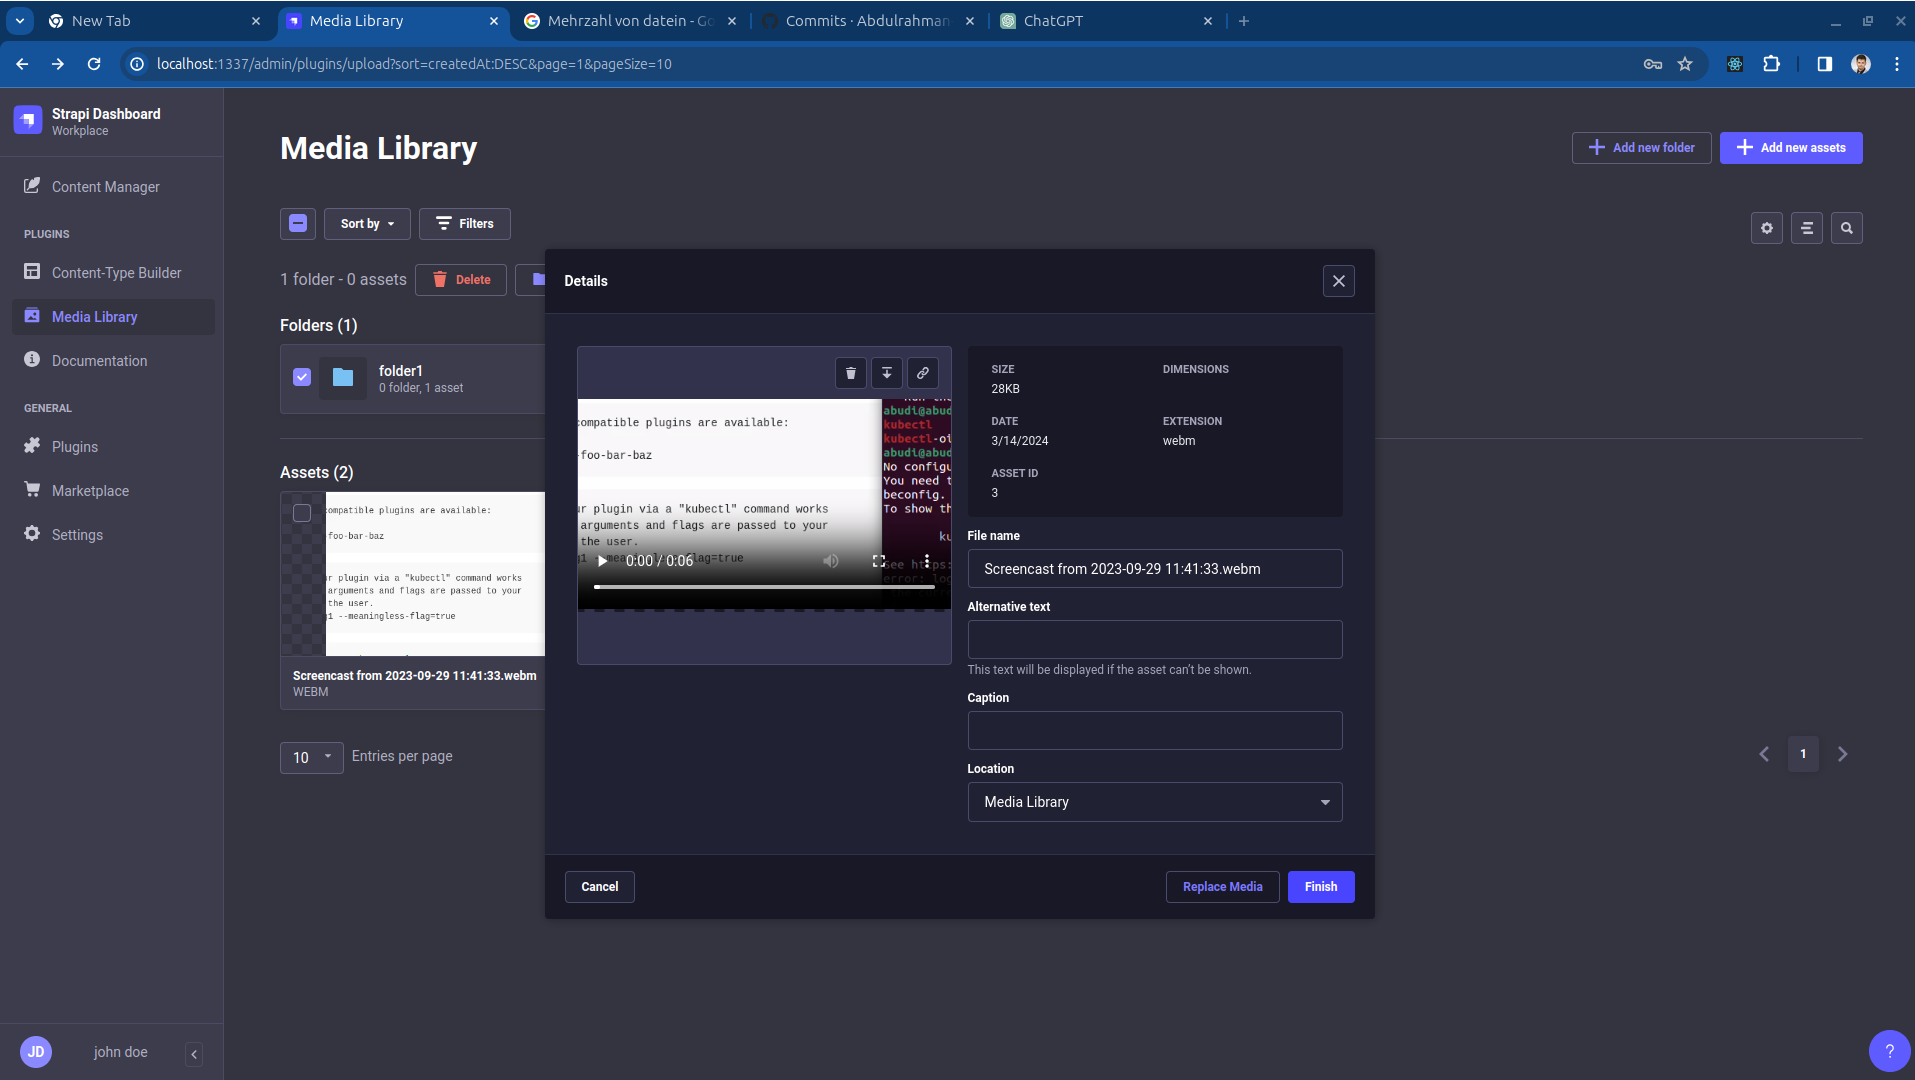
\includegraphics[width=\textwidth]{./pics/media-library.png}
  \caption{media-library}

\end{figure}

Es gibt auch die Möglichkeit, den Link einer Datei, wie zum Beispiel ein Video aus YouTube, in der Media Library 
einzubetten. Allerdings ist diese Funktion nur bei der aktuellsten Version leicht anwendbar. Bei älteren Versionen 
ist die Umkonfigurierung des Reverse Proxys des Systems notwendig. Sonstige Probleme mit lizenzfreien Inhalten 
sind dann nicht vom System zu lösen, sondern vom Content-Manager.
\cite{url-upload-problem}


% Beispiele dafür sind:

% \begin{itemize}
%     \item \textbf{RE}presentational \textbf{S}tate \textbf{T}ransfer (REST)- bzw. \textbf{G}raph \textbf{Q}uery \textbf{L}anguage (Graphql)-Schnittstellen
%     \item Logik für die Authentifizierung
%     \item \textbf{C}reate, \textbf{R}ead, \textbf{U}pdate und \textbf{D}elete (CRUD)
%           Funktionalitäten jeder Business Entität
% \end{itemize}


\section{Firebase App Distribution}

''Firebase App Distribution'' macht die Verteilung
Ihrer Apps an vertrauenswürdige Tester problemlos. Indem Sie Ihre Apps schnell
auf die Geräte der Tester übertragen, können Sie frühzeitig und häufig
Feedback einholen.
Und wenn Sie Crashlytics in Ihren Apps verwenden, erhalten Sie automatisch Stabilitätsmetriken für alle Ihre Builds, sodass Sie wissen, wann Sie zur Auslieferung bereit sind.''\cite{fire-base-app-distribution}

Der Vorteil von Firebase App Distribution ist,
dass man die Applikation auf dem eigenen Mobilgerät ausprobieren kann,
ohne die App auf dem Play Store bzw. App Store hochladen zu müssen.